\section{FOUR-SHIP TACTICS}
\label{sec:ttp_aa:tactics_4ship}

\begin{tcoloritemize}
    \blueitem[Flight / Four-Ship]
    Combination of 2 elements to a single four-ship or ``flight''.
    Standard group size for planning \& tasking purposes. 
    Allows flight to split into 2 groups while maintaining elements for mutual support
\end{tcoloritemize}

\subsection{FLIGHT RESPONSIBILITIES}

\begin{tcoloritemize}
    \blueitem[1 --- Flight Lead]
    \begin{itemize}
        \item primary planner, decision maker
        \item primary navigation, radar lookout
    \end{itemize}
    
    \blueitem[2 --- Wingman]
    \begin{itemize}
        \item maintain formation
        \item visual lookout
        \item radar / sensor awarness
        \item navigation \& position awarness
    \end{itemize}
    \blueitem[3 --- Element Lead]
    \begin{itemize}
        \item maintain formation
        \item secondary planner, decision maker
        \item secondary navigation, radar lookout
    \end{itemize}

    \blueitem[4 --- Wingman]
    Same as 2

\end{tcoloritemize}

\clearpage

\subsection{OFFENSIVE TACTICS}

\begin{tcoloritemize}
    \blueitem[Wall]
    Flight goes line abreast, 
    reference \cref{subsec:supp_fig:form:4ship,fig:supp_fig:form:4shiplab}
    for formation

    \bigskip
    \textbf{Advantages}
    \begin{itemize}
        \item \textbf{maximizes simultaneous weapon employment capability of flight}
        \item maximizes sensor coverage / overlap
    \end{itemize}

    \textbf{Disadvantages}
    \begin{itemize}
        \item difficult to maintain formation
        \item rapid geographic displacement, 
        not suited to holding/protecting area
    \end{itemize}
    
    \textbf{Typical Use Cases}
    \begin{itemize}
        \item Sweep --- clear airspace of threats
        \item Escort --- sanitize airspace in front of friendlies
    \end{itemize}
    \hfill\textbf{see \cref{fig:ttp_aa:4ship:offensive:wall}}
\end{tcoloritemize}

\begin{figure}[htbp]
    \centering
    \begin{tikzpicture}[figstyle]

        % coordinates
        \coordinate (lead_lead) at (0,0);
        \coordinate (lead_wing) at (-15,0);
        \coordinate (elem_lead) at (15,0);
        \coordinate (elem_wing) at (30,0);
        \coordinate (bandit) at (7.5,40);
        \coordinate (bandit_wing) at (2.5,45);

        % fighter wez
        \draw[fill=color2!15] 
            \foreach \n in {lead_lead, lead_wing, elem_lead, elem_wing} {
                (\n) -- ++(60:25) arc (60:120:25) -- cycle
            };

        % fighters
        \foreach \n in {lead_lead, lead_wing, elem_lead, elem_wing} {
            \node[] (\n_fig) at (\n) {
                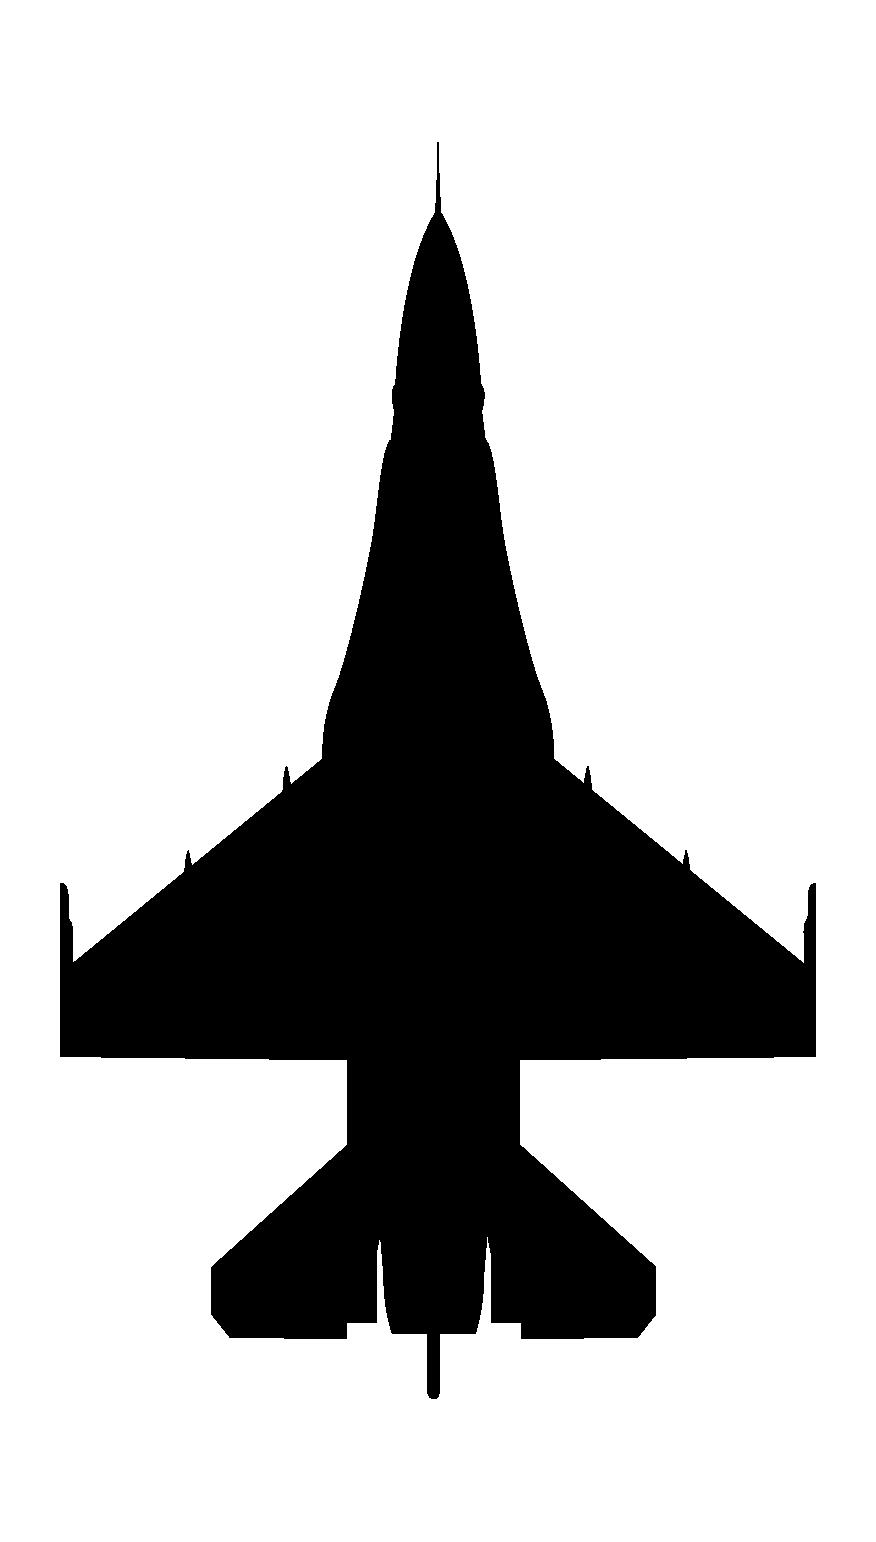
\includegraphics[
                    width=7.5mm,
                ]{diagrams/aircraft/silhouette_f16_top.pdf}
            };
        }

    \end{tikzpicture}
    \caption{Four-ship wall tactics}%
    \label{fig:ttp_aa:4ship:offensive:wall}
\end{figure}

\notebox{
    \small
    \begin{itemize}
        \item Wall tactics are \textbf{NOT} limited to four-ship, 
        8-ship wall also typical, depends on threat environment
        \item Modification of formation to spread or fluid-four,
        shown in \cref{fig:supp_fig:form:spread,fig:supp_fig:form:fluidfour} respectively,
        can vastly simplify maintaining formation
    \end{itemize}
}

\clearpage

\begin{tcoloritemize}
    \blueitem[Grinder]
    Flight splits into elements, enter racetrack pattern

    \bigskip
    \textbf{Advantages}
    \begin{itemize}
        \item \textbf{at least one element hot}
        \item grinder remains geographically stationary
        \item continual sensor coverage along grinder axis
        \item cold element available for delouse
    \end{itemize}

    \textbf{Disadvantages}
    \begin{itemize}
        \item reduced simultaneous weapon employment \& sensor coverage capability
        \item difficult to set up \& regroup to four-ship
    \end{itemize}

    \textbf{Typical Use Cases} 
    \begin{itemize}
        \item CAP --- Combat Air Patrol, protection of geographic area for prolonged vulnerability period
        \item HAVCAP --- High Asset Value CAP, protection of high value assets (AWACS, tanker, EW)
    \end{itemize}
    
    \hfill\textbf{see \cref{fig:ttp_aa:4ship:offensive:grinder}}

    \blueitem[Hot Element \break Priorities]
    \begin{itemize}
        \item sorting, targeting
        \item radio / communications
    \end{itemize}

    \blueitem[Cold Element \break Priorities]
    \begin{itemize}
        \item building situational awarness
        \item listen for comms from hot element
        \item know when to turn in
    \end{itemize}
\end{tcoloritemize}

\notebox{
    \small%
    Grinder tactics do \textbf{NOT} necessarily require four-ship, 
    can be employed by a single element. 
    However, most common for four-ship.
}

\begin{figure}[htbp]
    \centering
    \begin{tikzpicture}[figstyle]

        % coordinates
        \coordinate (lead_hot) at (0,0);
        \coordinate (wing_hot) at (-10,0);
        \coordinate (lead_cold) at ($(lead_hot) + (20,-40)$);
        \coordinate (wing_cold) at ($(wing_hot) + (20,-40)$);
        \coordinate (bandit) at (0,40);
        \coordinate (bandit_wing) at (-10,45);

        % bandit wez
        \draw[fill=red!40] 
        (bandit_wing) -- ++(-60:15) arc (-60:-120:15) -- (bandit_wing);
        \draw[fill=red!40] 
        (bandit) -- ++(-60:15) arc (-60:-120:15) -- (bandit);

        % \draw[fill=color2!15] 
        % (lead_hot) -- ++(87:47) arc (87:93:47) -- (lead_hot);
        % \draw[fill=color2!15] 
        % (wing_hot) -- ++(87:52) arc (87:93:52) -- (wing_hot);

        % fighters
        \node[below] (lead_hot_fig) at (lead_hot) {
            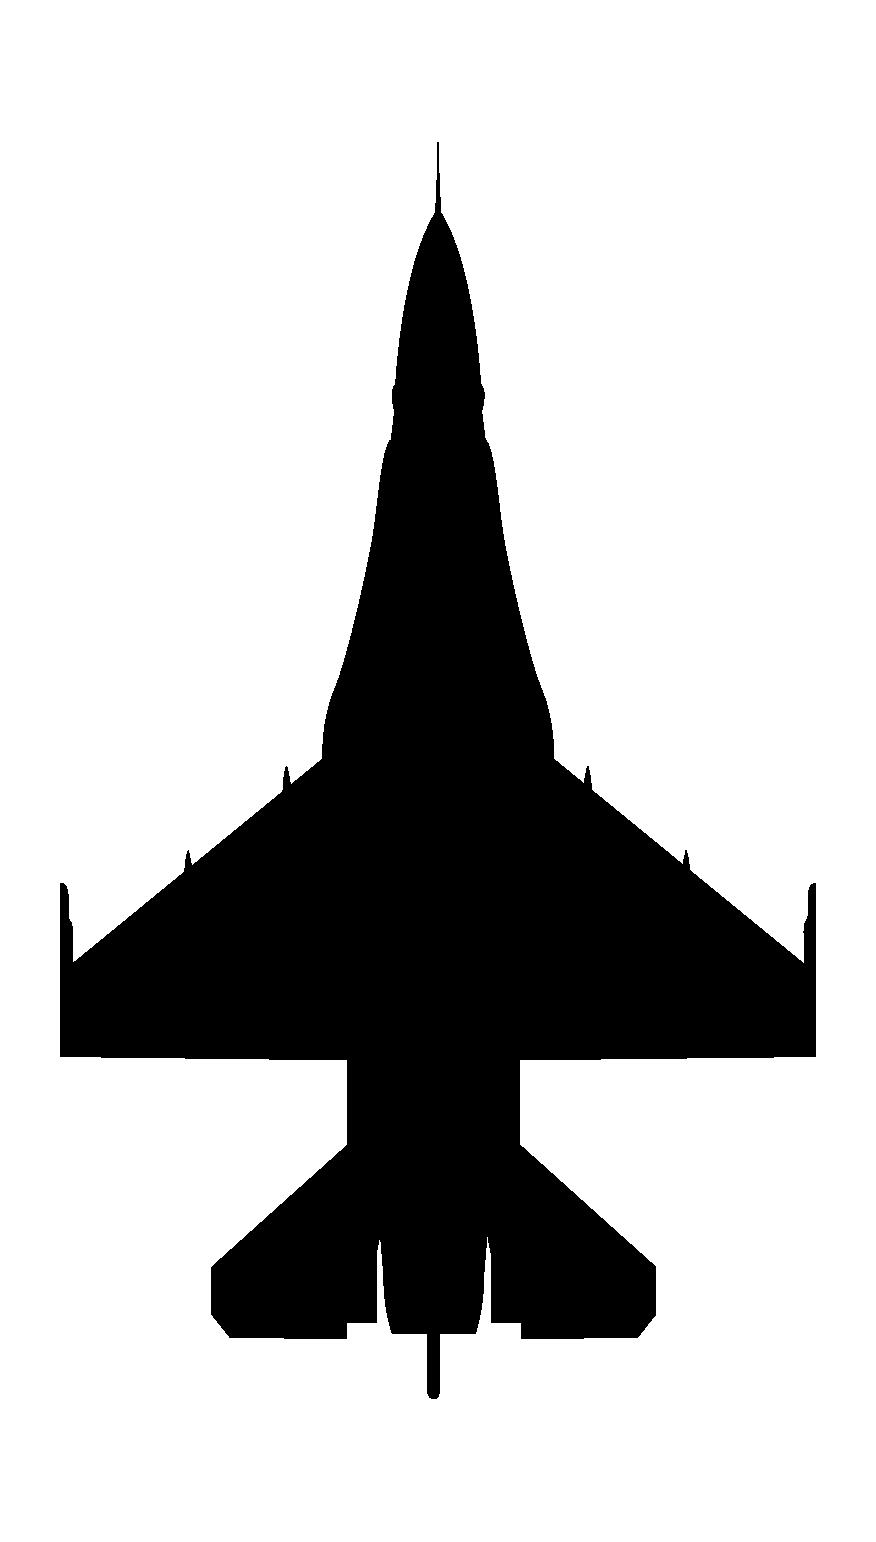
\includegraphics[
                width=7.5mm,
            ]{diagrams/aircraft/silhouette_f16_top.pdf}
        };
        \node[below] (wing_hot_fig) at (wing_hot) {
            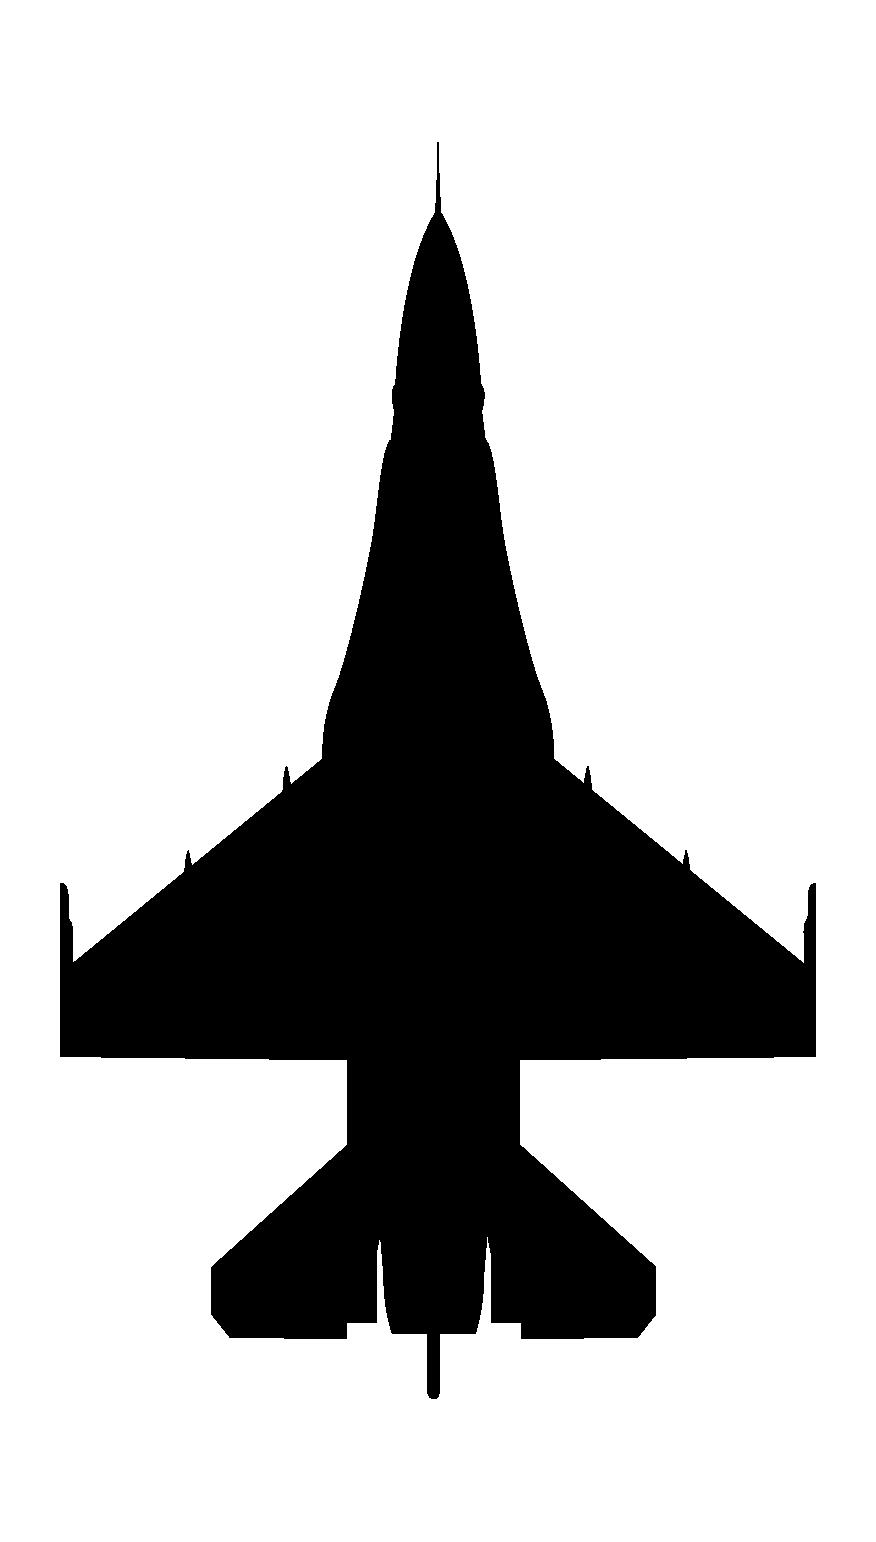
\includegraphics[
                width=7.5mm,
            ]{diagrams/aircraft/silhouette_f16_top.pdf}
        };
        \node[below, rotate=180] (lead_cold_fig) at (lead_cold) {
            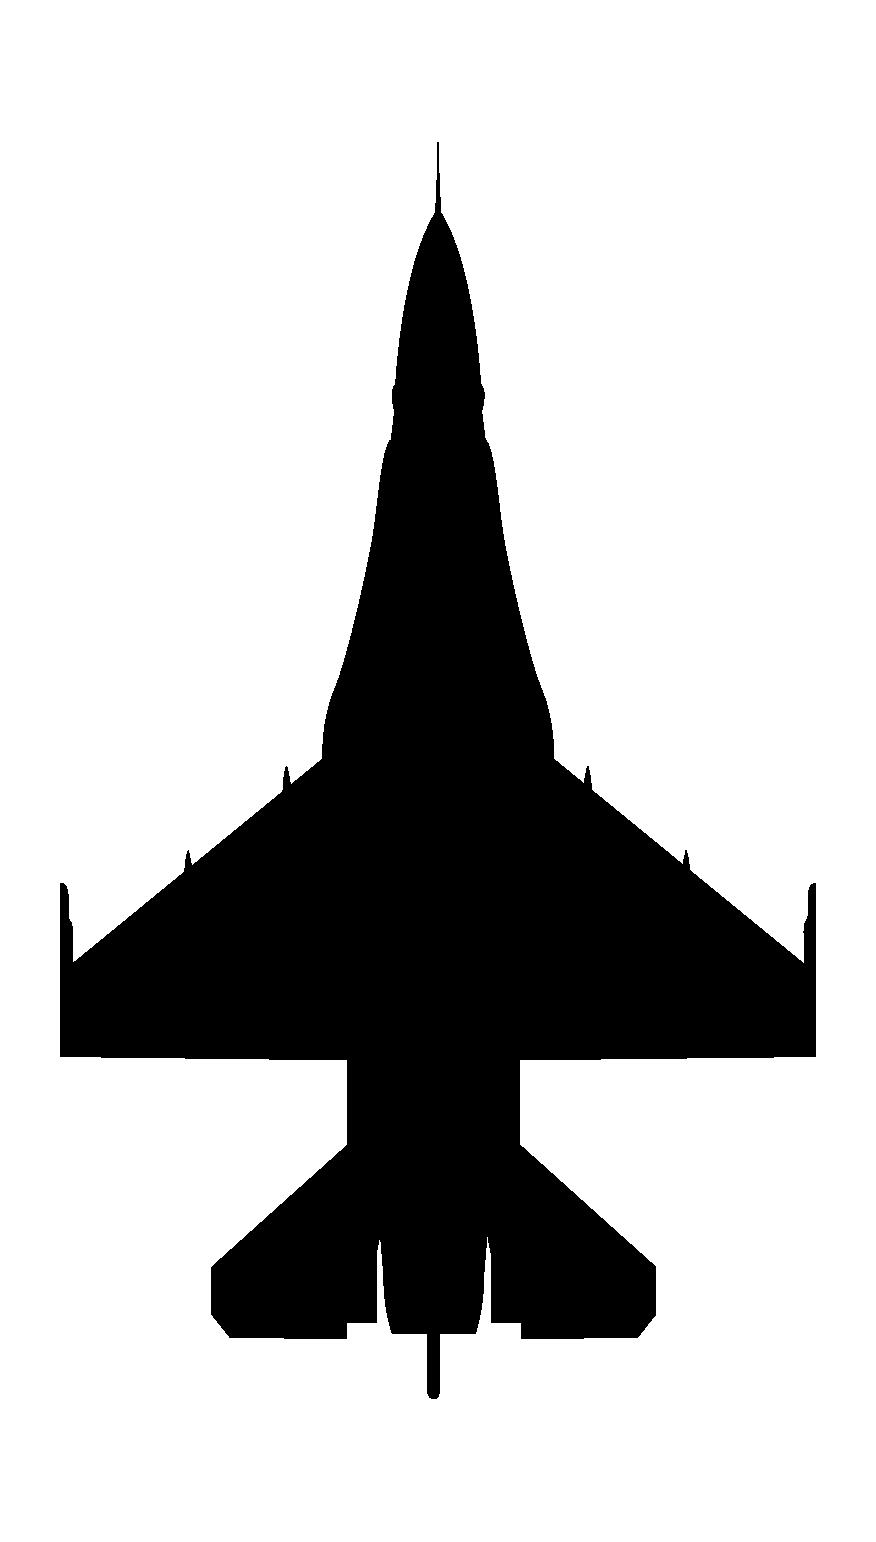
\includegraphics[
                width=7.5mm,
            ]{diagrams/aircraft/silhouette_f16_top.pdf}
        };
        \node[below, rotate=180] (wing_cold_fig) at (wing_cold) {
            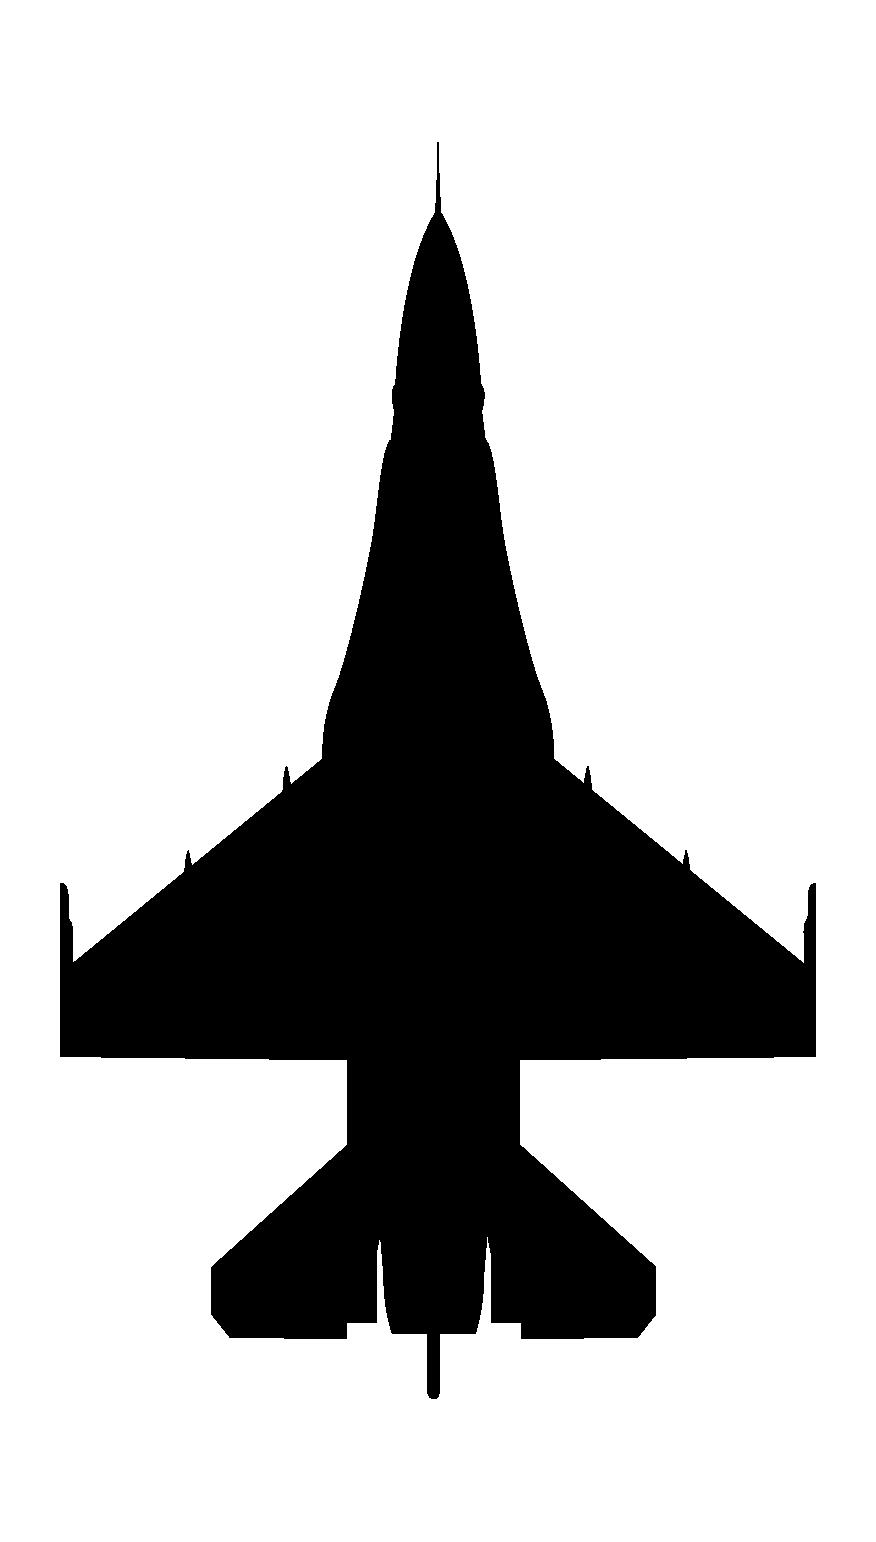
\includegraphics[
                width=7.5mm,
            ]{diagrams/aircraft/silhouette_f16_top.pdf}
        };
        
        \foreach \n in {lead, wing} {
            \draw[->] 
                (\n_hot) 
                -- ++(0,5)
                arc (180:0:10) 
                -- (\n_cold_fig.south);
            \draw[->] 
                (\n_cold) 
                -- ++(0,-5)
                arc (0:-180:10) 
                -- (\n_hot_fig.south);
        }

        % bandit
        \node[] (bandit_fig) at (bandit) {
            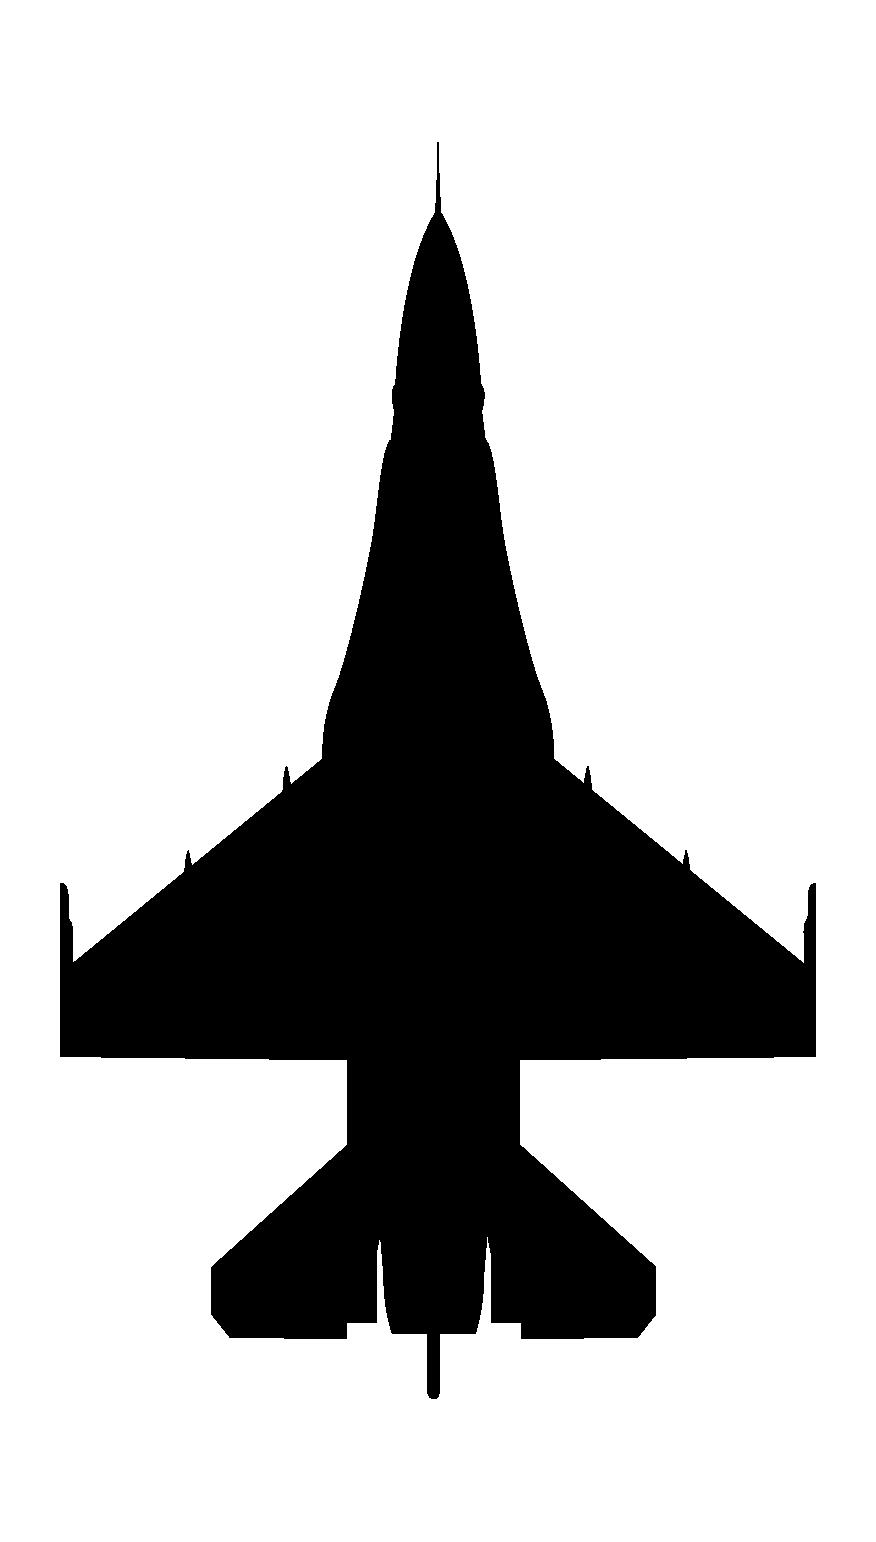
\includegraphics[
                    angle=180,
                    width=7.5mm,
            ]{diagrams/aircraft/silhouette_f16_top.pdf}
        };
        \node[] at (bandit_wing) {
            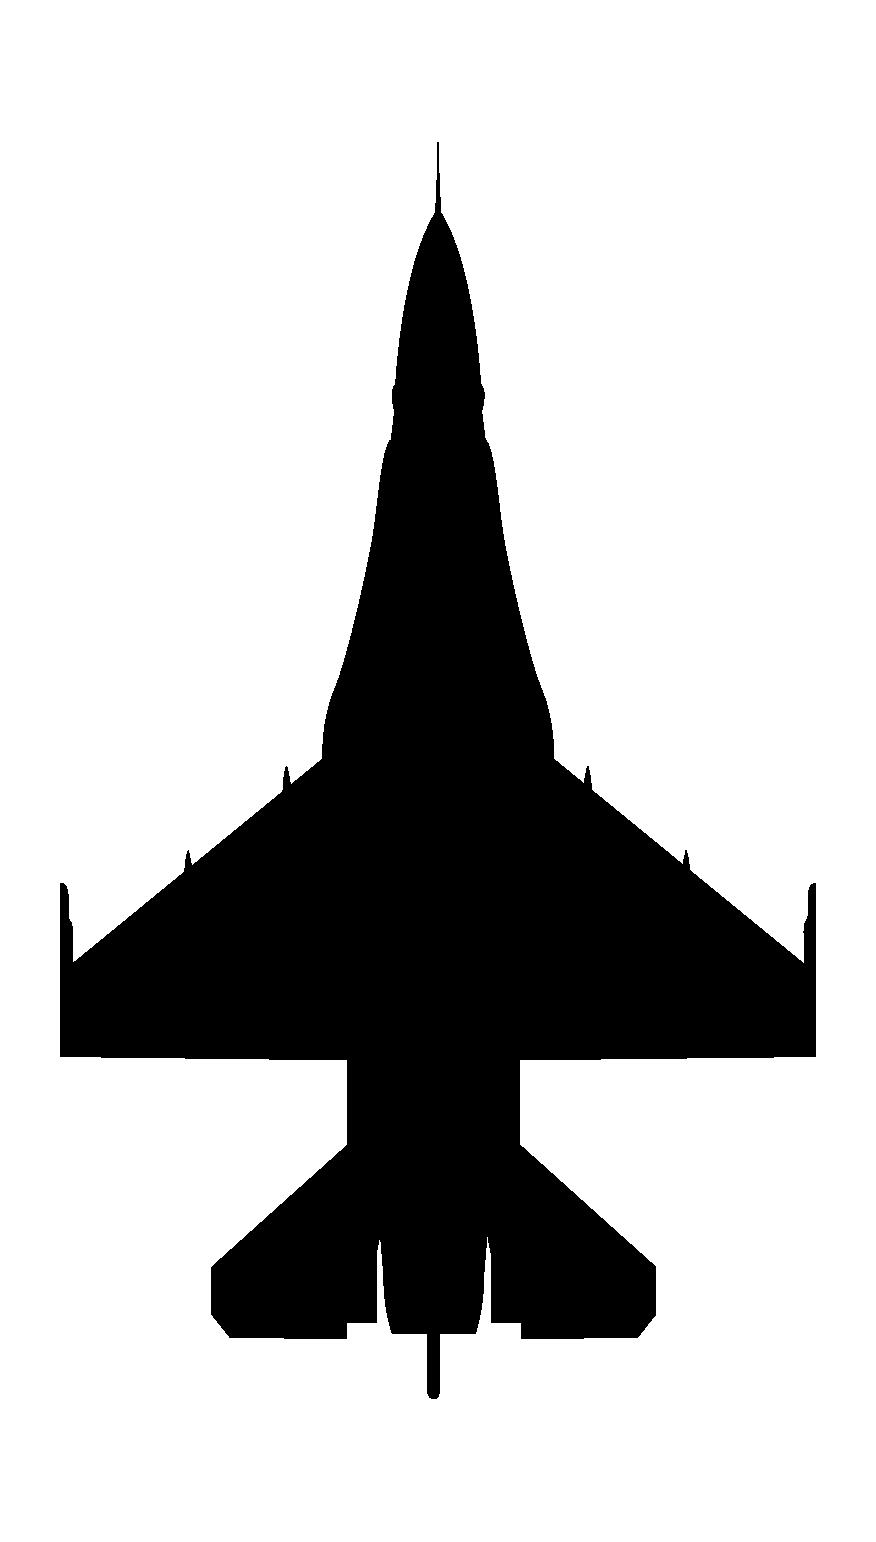
\includegraphics[
                    angle=180,
                    width=7.5mm,
            ]{diagrams/aircraft/silhouette_f16_top.pdf}
        };

        % labels
        \node[font=\small, align=right, left] at (wing_hot_fig.west) {Hot \\ Element};
        \node[font=\small, align=left, right] at (lead_cold_fig.west) {Cold \\ Element};
        \node[font=\small, right] at (bandit_fig.east) {Bandits};

    \end{tikzpicture}
    \caption{Four-ship grinder tactics}%
    \label{fig:ttp_aa:4ship:offensive:grinder}
\end{figure}

\clearpage

\subsection{DEFENSIVE TACTICS}

\begin{tcoloritemize}
    \blueitem[Delouse] 
    Non-engaged element turns hot on bandits spiking other elment,
    spiked element continues cold.

    \bigskip
    \textbf{Advantages}
    \begin{itemize}
        \item clears spiked element/friendlies
        \item forces bandits defensive
    \end{itemize}

    \textbf{Typical Use Cases}
    \begin{itemize}
        \item cold element in grinder clears hot element post-engagement
        \item friendly aircraft request delouse from fighters on egress / after aborting
    \end{itemize}

    \hfill\textbf{see \cref{fig:ttp_aa:4ship:defensive:delouse}}
\end{tcoloritemize}

\notebox{
    \small Delouse is \textbf{NOT} restricted to four-ship, 
    or to within own flight, 
    it is a general defensive tactic to clear friendlies when recommitting is not available.
}

\begin{figure}[htbp]
    \centering
    \begin{tikzpicture}[figstyle]

        % coordinates
        \coordinate (spiked_lead) at (0,0);
        \coordinate (spiked_wing) at ($(spiked_lead) + (-10,5)$);
        \coordinate (naked_lead) at (60, 10);
        \coordinate (naked_wing) at ($(naked_lead) + (-10,5)$);
        \coordinate (bandit_lead) at (0,40);
        \coordinate (bandit_wing) at ($(bandit_lead) + (-10,5)$);

        % bandit
        \foreach \n in {bandit_lead, bandit_wing}
        {
            \draw[fill=red!40] 
            (\n) -- ++(-87:42) arc (-87:-93:42) -- cycle;
            \node[] (\n_fig) at (\n) {
            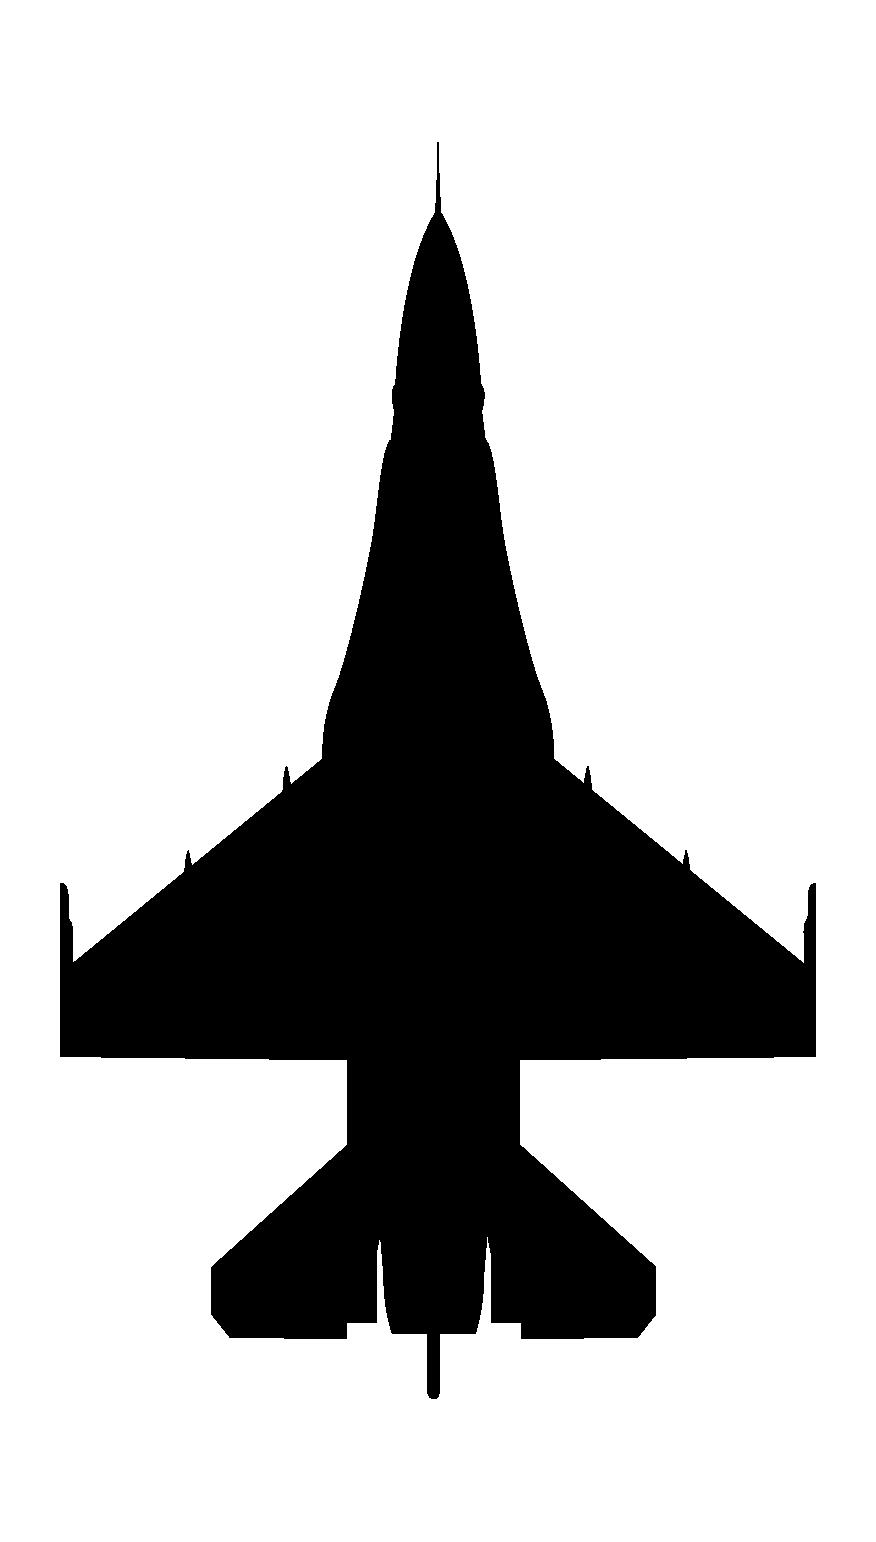
\includegraphics[
                    angle=180,
                    width=7.5mm,
            ]{diagrams/aircraft/silhouette_f16_top.pdf}
        };
        }

        % fighters
        \foreach \n in {spiked_lead, spiked_wing, naked_lead, naked_wing}
        {
            \node[rotate=180] (\n_fig) at (\n) {
                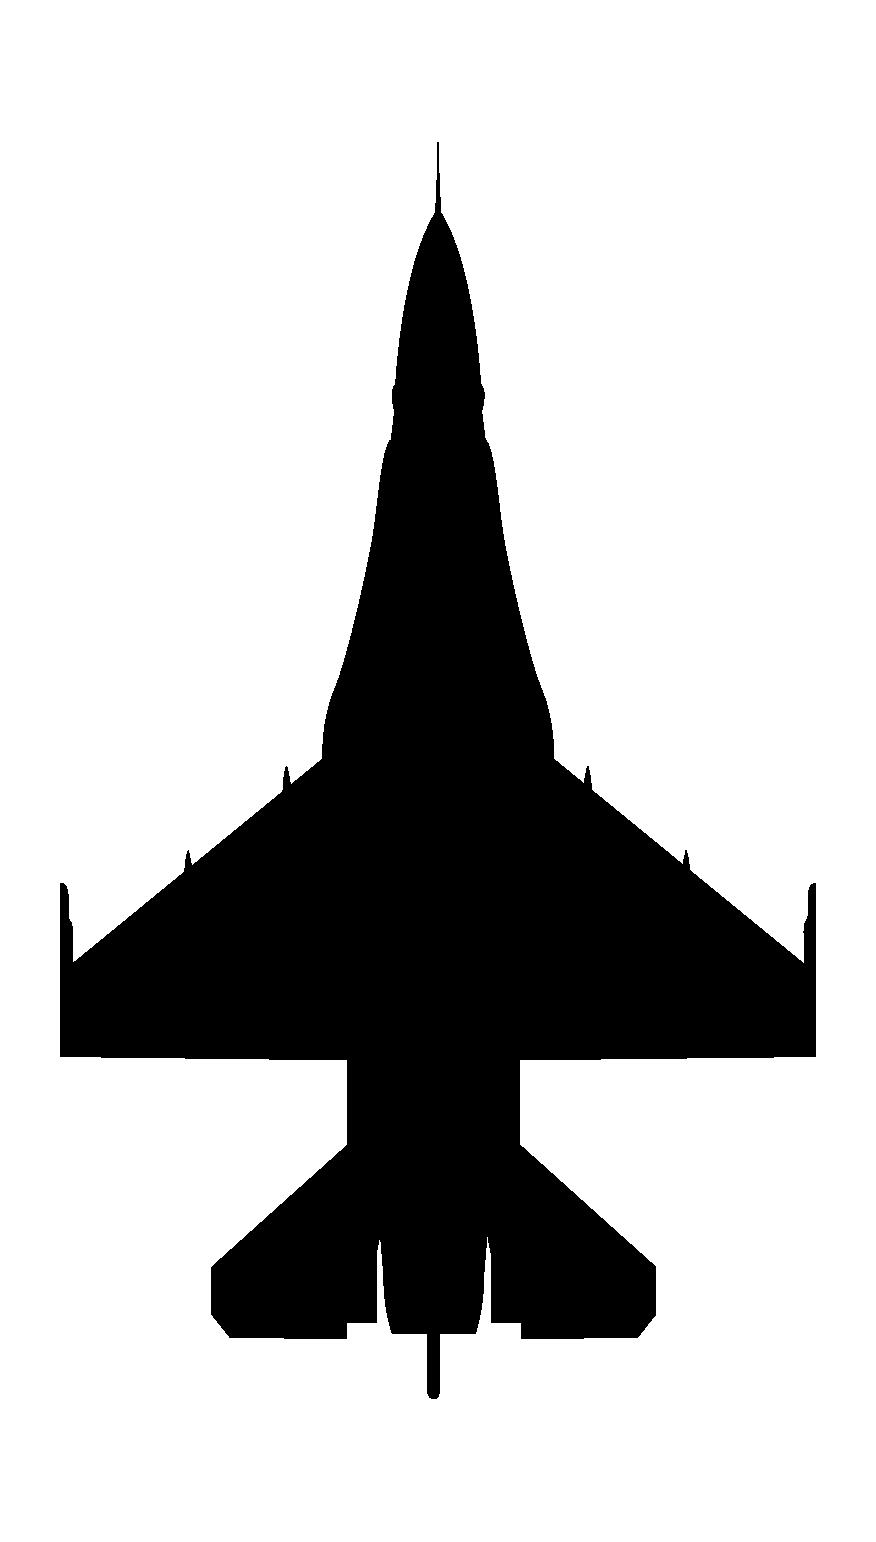
\includegraphics[
                    width=7.5mm,
                ]{diagrams/aircraft/silhouette_f16_top.pdf}
            };
        }

        % flightpath
        \draw[->]
            (spiked_lead_fig.north) 
            -- ++(0,-10);
        \draw[->]
            (spiked_wing_fig.north) 
            -- ++(0,-10);
        \draw[->]
            (naked_lead_fig.north) 
            -- ++(0,-5)
            arc (0:-150:10)
            -- ++(120:20);
        \draw[->]
            (naked_wing_fig.north) 
            -- ++(0,-10)
            arc (0:-150:10)
            -- ++(120:20);

        % labels
        \node[font=\small, align=right, left] at (spiked_wing_fig.east) {Spiked \\ Element};
        \node[font=\small, align=left, right] at (naked_lead_fig.west) {Naked \\ Element};
        \node[font=\small, right] at (bandit_lead_fig.east) {Bandits};

    \end{tikzpicture}
    \caption{Four-ship delouse}%
    \label{fig:ttp_aa:4ship:defensive:delouse}
\end{figure}